\documentclass{article}
%\usepackage[utf8]{inputenc}

\title{Spatio-temporal prediction of NO2 in Madrid, Spain}
\author{Meng Lu} 

\usepackage{natbib}
\usepackage{graphicx}
\usepackage{cleveref}
\usepackage{booktabs}
\usepackage{todonotes}


\begin{document}

\maketitle


\section{Introduction}

 

Nitrogen dioxide is a significant health risk. Forecasting NO2 to the next few days at an intra-urban level provide opportunities to reduce personal exposures. Numerical air pollution models accounting for chemical reactions and air transportation have been developed to predict urban air pollution.
The MACC (monitoring atmospheric composition and climate) project \cite{MACC} of the Copernicus Atmosphere Monitoring Service (CAMS) forecast air pollution to the next 96 hours. The model, model simulation and forecasts from MACC project are respectively referred to as MACC model, simulation, and forecast. The spatial resolution of MACC forecasts is 0.1 degree, which is coarse for a city scale. In addition, the MACC forecasts are not calibrated with local sensor measurements. This study focus on air pollution prediction in Madrid, Spain. The 24 ground air pollution stations operated for several years in Madrid provide dense temporal records to downscale MACC forecasts. 

Our study focus on NO2 forecasting as NO2 is measured by the largest number of air quality stations. The objective of this study is to use the historical station measurements and their spatiotemporal correlations to improve MACC forecasts. We firstly interpolate the MACC forecast to a city grid of 0.05 by 0.05 degree resolution. Then, we integrate temporal and spatial correlation and 3-year historical records of station  measurements time series into the MACC predictions. The station measurements are treated as "real measurements" and as a dependent variable in all the regressions, specifically, A series of linear regression, geostatistical and random forest methods are evaluated and compared to identify predict NO2 to the next 12 hours over Madrid city. 

\begin{enumerate} 
    \item  Modelling the time series characters of state sensor measurements and the relationship between MACC and station sensor measurements using linear, polynomial regression and GAM (general additive model). 
     
    \item  Modelling the spatial correlation of the residuals of a linear regression model with sensor measurements as dependent variables and interpolated MACC as independent variables by applying universal kriging. 
    
    \item  Exploring non-linear relationship between station sensor measurements and the MACC simulations, time series patterns (e.g. harmonic terms and time of day, day of year) with random forest regression.
\end{enumerate}

 % The linear regression model considers linear and non-linear relationships between historical station measurements, MACC simulations and temporal variations, without considering spatial correlation. The model 3 considers a universal kriging model to integrate spatial correlation and predict NO2. The model 4 trains a random forest model to predict NO2 using historical records of time series patterns and MACC simulations.  

%These three methods are evaluated and compared to each other.  




\section{Data and data preprocessing}
\label{sec:data}

Three years of hourly NO2 station measurements and MACC simulations are available. In total, there are 24 air quality measuring stations distributed in the city of Madrid, Spain %\todo{add a figure}. 
%These station measurements are used to train models and to validate the modelling results. 
\Cref {fig:sample} shows time series of half-day NO2 concentrations of three stations.  
%\todo{Add a
%  deeper description of the data (JLA)} \todo{ what is JLA?}

The spatial resolution of MACC data is 0.1 degree, and Madrid city grid 0.05 degree. We aggregated the hourly MACC and station measurements to half day (12 hours), which is the required temporal prediction resolution for the final product. The missing value of the station measurements are filled using spline interpolation. For the MACC simulation, two time steps of historical records are missing. The distribution of MACC forecast of NO2 and the measured NO2 are skewed Gaussian distribution (\cref
{fig:hist}).  

 

\begin{figure}[tbp]
 \center
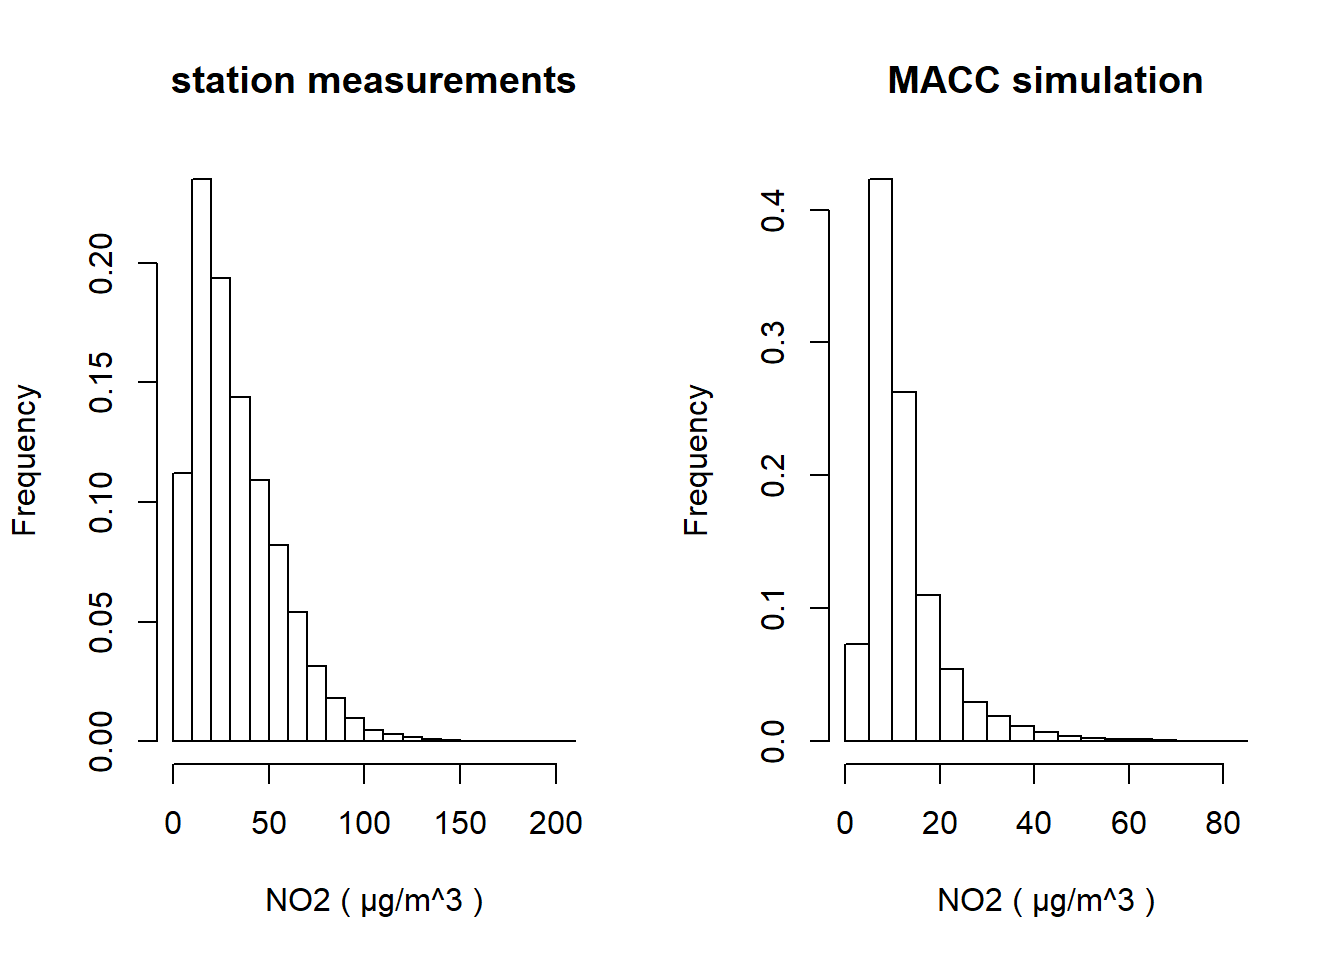
\includegraphics[scale = 0.8]{hist.png}
\caption{Histogram of station measurements (left) and MACC simulation (right)}
\label{fig:hist}
\end{figure}

\begin{figure}[tbp]
  \center
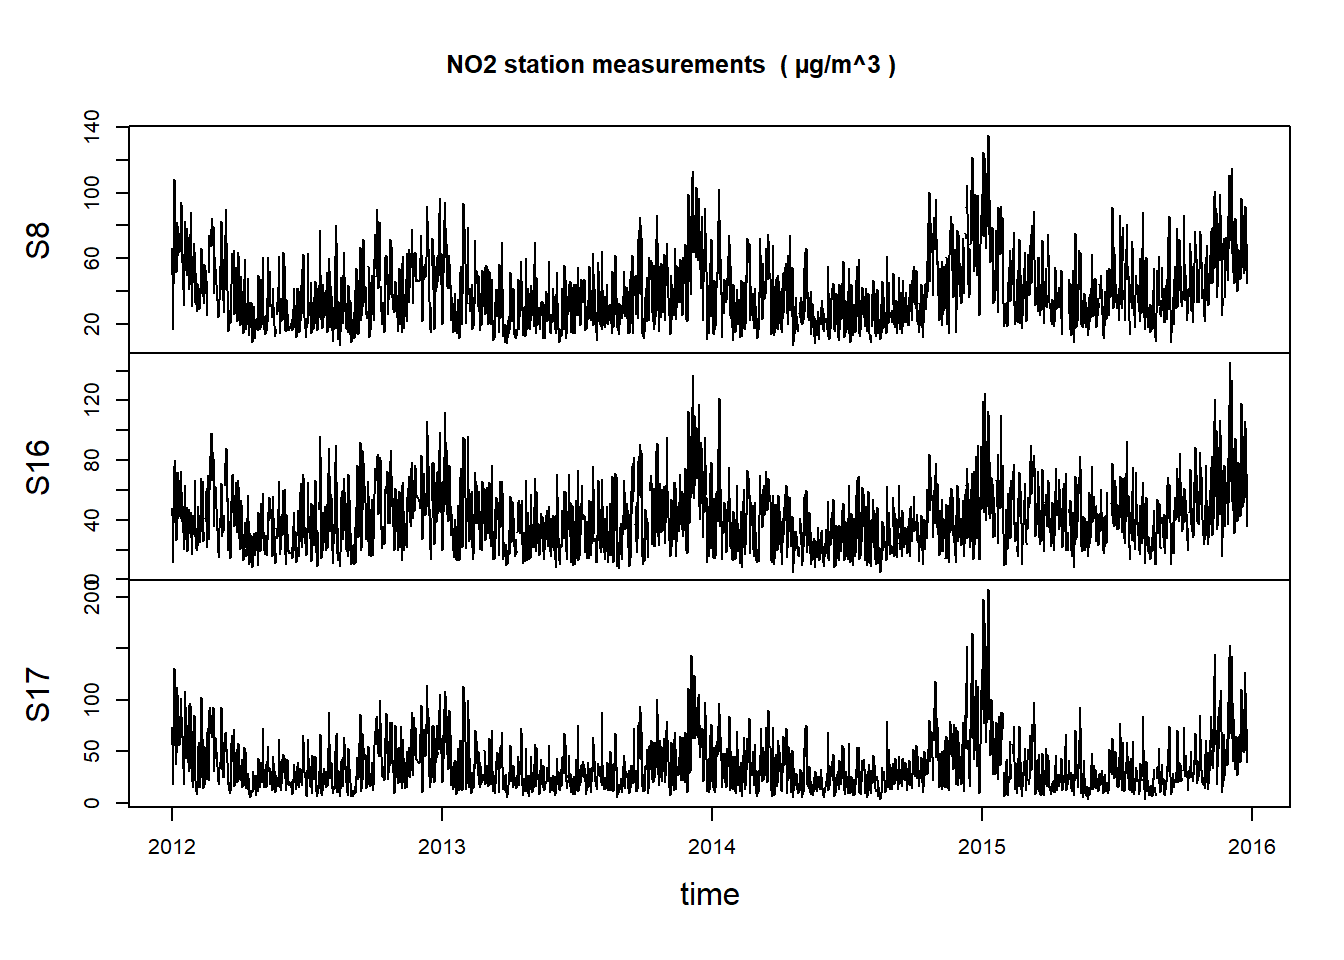
\includegraphics[scale = .8]{sample.png}
\caption{Halfday time series of NO2 measurements of stations with id 8, 17 and 16 (S8, 16, 17)}
\label{fig:sample}
\end{figure}

\section{Ordinary kriging of MACC simulation} 
 
The MACC provide prediction of the next half day, and strong spatial correlation are presented in the MACC simulations. The model 1 therefore interplote  MACC simulations to the city grid. In an attempt to use more information from historical MACC numerical predictions, we computed a pooled variogram \Cref{fig:vno2} from MACC forecasts of 200 sampled time stamps. The pooled variogram is calculated as averaged semivariance over the sampled time stamps os MACC simulations. An "ste" variogram model \citet[Matern, M. Stein’s parameterization,][]{automap} is automatically fitted with the initial parameters of nugget, sill and range set as \citet{automap} to the variogram and is used to interpolate MACC forecasts to the city grid and to each of the measuring stations.
 
\begin{figure}[tbp]
 \center
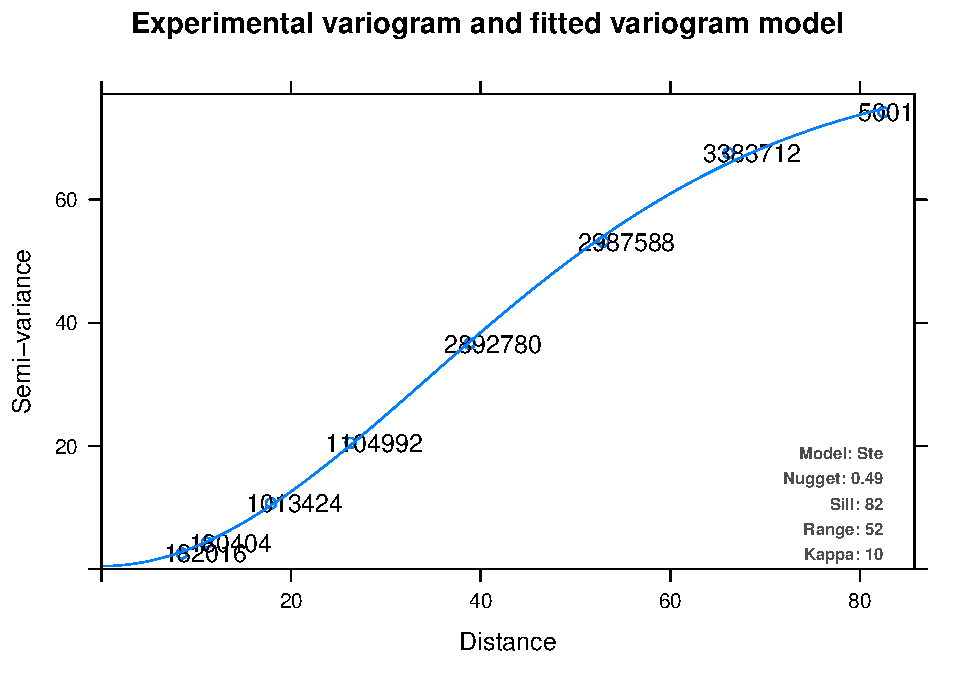
\includegraphics[scale = 0.8]{vno2.pdf}
\caption{ Pooled variogram and variogram model of half-day MACC simulated NO2 concentration.}
\label{fig:vno2}
\end{figure}

\section{Linear and nonlinear regression model .}
\subsection{method}
The models in this section investigate linear or non-linear relationship between MACC simulation and station measurements. Linear,
polynomial, and general additive models are attempted. (Adjusted) R square and model complexity were considered to select the best model. 
  
Five models are attempted to investigate the relationship between station measurements and spatially interpolated MACC
forecast. Model 2a and 2b and 2c are linear regression models. In model 2b, time of day (TOD) and harmonic terms are used as additional
independent variables. The models are built with station measurements and corresponding MACC simulations from 2012-01-01 to 2015-12-31 \cref{table:1}.

Based on the time series fluctuation pattern, the harmonic terms $|sin(2 \pi wt) + \phi|$, with
$w = 1 / (356 * 2 )$ are used to fit the half year positive
cyclical pattern\todo{It would be nice to justify this
  graphically.}. 34.8\% percent of variance could be explained by the MACC simulations, 38.2\% percent of variance could be explained with additional harmonic terms. 39 \% percent of variance could be explained with MACC simulations, harmonic terms, and TOD. 

\begin{figure}[tbp]
  \center
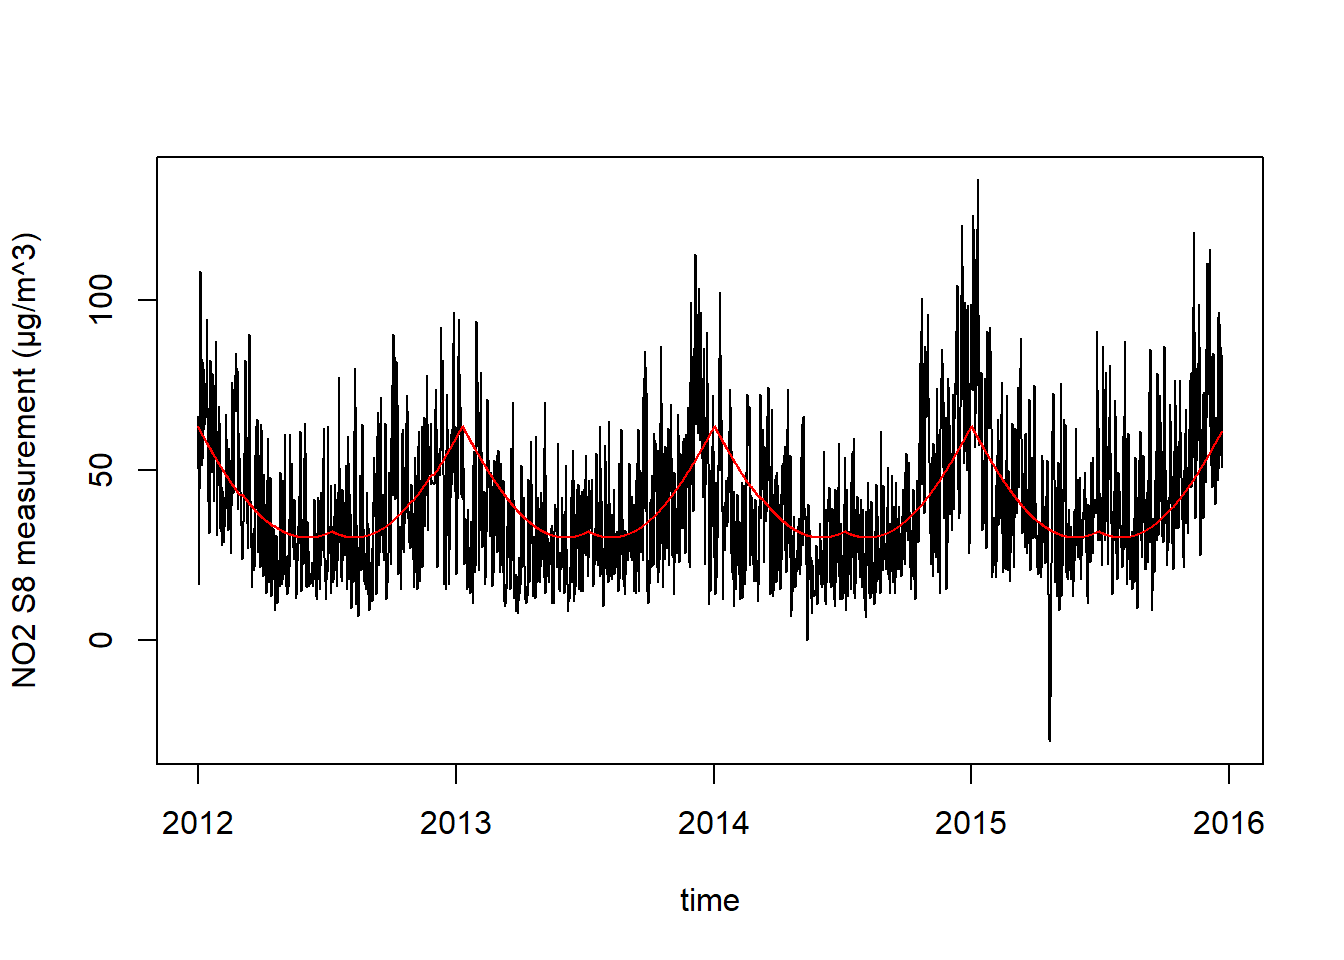
\includegraphics[scale = 0.6]{fit.png}
\caption{The harmonic terms (red) fitted to an NO2 time series. }
\label{fig:fit}
\end{figure}
 
 
\begin{table}[tbp]
\centering
\begin{tabular}{ c c c }
  \toprule
Model & Method & Independent variable\\ \midrule

2a &linear regression &MACC   \\
2a1 & second order polynomial & MACC \\  
2a2 & third order polynomial & MACC   \\ 

2b &linear regression & MACC, Harmonics   \\
2c &linear regression & MACC, Harmonics, TOD  \\
2d & general additive model & MACC  \\  \bottomrule
\end{tabular}
\caption{ Linear and non-linear regression models and the independent variables of the model. TOD: time of day. } 
\label{table:1}
\end{table}

\begin{figure}[tbp]
  \center
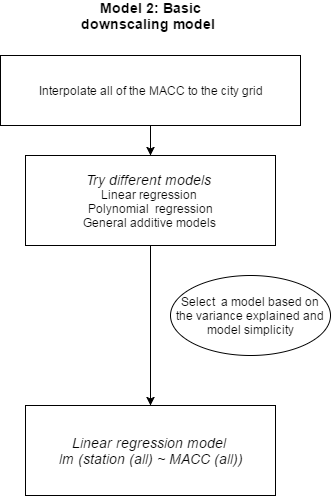
\includegraphics[scale = 0.4]{diaM2.png}
\caption{The workflow of model 2. The model 2a, which is a linear
  regression model with MACC as independent variable has obtained the
  best results and used to compare with models using other methods. }
\label{fig:LR}
\end{figure}

Because the linear regression result shows using of temporal characters does not improve the results, we only investigated non-linear relationship between MACC and station measurements. 
\todo[inline]{A question rises when reading Table \ref{table:1}: why
  we didn't use the TOD and the harmonics in 2c1, 2c2 and 2d? And why
  didn't we use the day of the week (DOW) and day of the year (DOY)
  variables? It is known that the NO2 series shows a weekly and yearly
  cycle. We should be prepared to answer it in revision phase (or
  solve it beforehand).}

 

\section{Universal Kriging}

The basic downscaling models do not utilise spatial information. Universal Kriging is used to utilise spatial correlations. We computed and observed spaital correlation in the residual variograms %1) with 
using MACC simulations as a regressor
%, and 2) with residual variograms with MACC simulations and locations as regressors.



\subsection{Universal kriging models}

\begin{figure}[tbp]
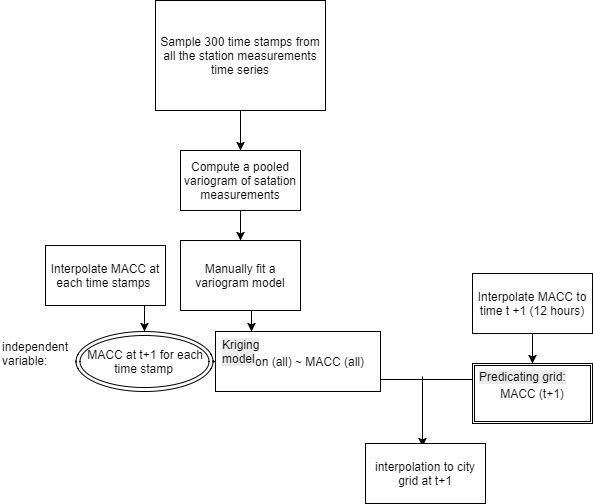
\includegraphics[width=\columnwidth]{diaM3.png}
\caption{Flowchart for the universal krigging models. The variogram model is fitted to the residuals of a linear regression model fit to all the half-day historical
  station measurements (about 3 years of data). Then the MACC simulations of the halfday to be predicted is interpolated to the city grid to predict air quality.}
\label{fig:UK}
\end{figure}

\Cref{fig:UK} shows the workflow the model 3. A pooled variogram is calculated randomly sampled time stamps. We used data from all the
locations and times to fit the linear regression model, and applied
Kriging to the linear regression model residuals.

\todo[inline]{I think we will have to make this section more detailed,
stressing the justification for the decisions we made. - I will discuss about the model 3a and 3b in discussion} 

\subsection{Pooled residual variogram}

In an attempt to draw more spatial information, the residual variogram  \Cref{fig:variogram} is calculated as the average semivariance of the residuals of a linear regression model with MACC simulations from 300 sampled spatiotemporal points. \Cref{fig:variogram} shows the spatial correlation is not revealed from the station measurements. 


\begin{figure}[tbp]
  \center
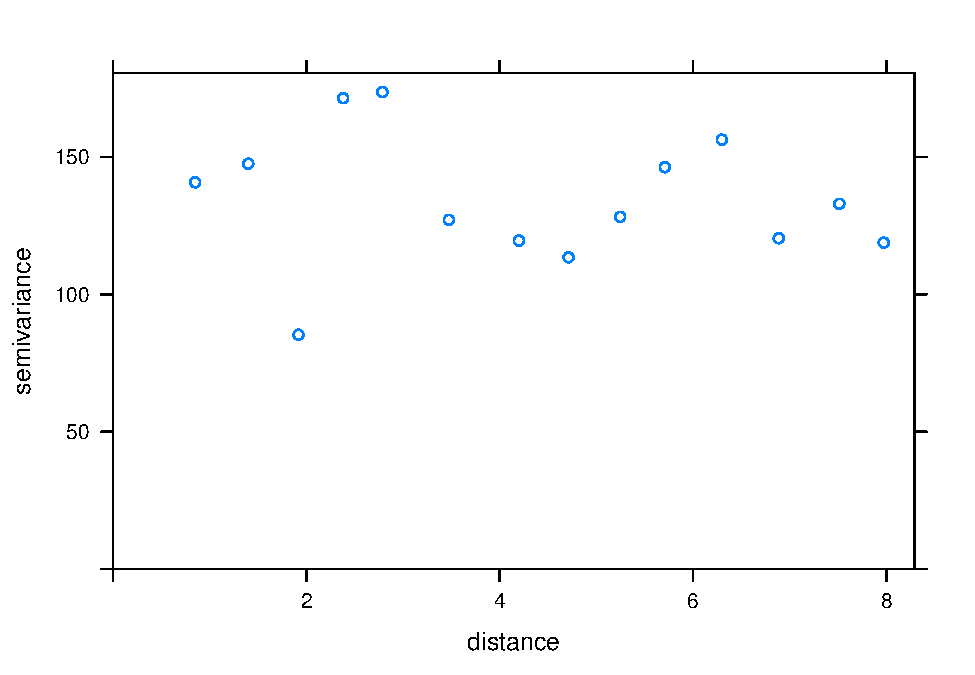
\includegraphics[scale = 0.4]{variogram.pdf}
\caption{The variogram of station measurements }
\label{fig:variogram}
\end{figure}




\subsection{Manually fitting a variogram model to the variogram for prediction}

Though spatial correlation is not revealed from the station measurements, it is possible that the spatial correlation could be shown if the stations are more densely sampled with closer distances. To draw the spatial information, we manually assigned the sill and
nugget of a variogram model assuming assuming spatial correlation exists within shorter distances. 
After manually fitting the variogram model, we applied universal kriging using this variogram model to interpolate station measurements to the city grid and forecast to the next halfday.



\section{Random forest}
\label{sec:rf}

\begin{table}[tbp]
\centering
\begin{tabular}{ c c  }
Model &  Independent variable\\ \hline 

 4.1 & MACC simulations, DOY, harmonic term, TOD \\
 4.2a & MACC simulations, DOY, TOD (factors) \\
 4.2b & MACC simulations, DOY (factors), TOD (factors) \\ 
 4.3 & DOY, MACC simulations \\
 4.4 & MACC simulations  \\  
 4.5 & downscaled MACC simulations from model 2a, DOY \\ \hline
\end{tabular}
\caption{Independent variables used in each model. DOY: day of year, TOD: time of day  } 
\label{table:rf}
\end{table}

To find a relationship between NO2 station measurements, MACC simulation and other temporal
variables, we used the random forest method. The MACC simulation, day of year (DOY),
time of day (TOD), and the NO2 predicted using model 2a are used as potential variables of the random forest.

Table \ref{table:rf} shows the variables that are used in each
model. The harmonic term that is used in model 2
($|sin(2 \pi wt) + \phi|$) is used in model 4.1. The model 4.2b treats DOY as factors (multiple variables) and model 4.2a treats the DOY as numbers (one variable). 

After the models are trained, the interpolated MACC simulations from model 1, the downsclared MACC simulations from model 2a, are used in the corresponding models for prediction. 


\todo[inline]{In this section it is not very clear how did we use the
  spatial information, if we did at all. A diagram would be useful.}
 


\section{Accuracy assessment}


For model 1, 2, and 4, half of the station measurements (i.e. the first 1.5 years of half-day station measurements,
in total 1420 observations) are used to train the model. The other half of 
the station measurements (i.e. the last 1.5 years of of half-day station measurements, in total
1428 observations) are used to test the model.  

For the model 3, as the universal kriging model uses the station measurements for interpolation, the differences between the predictions and station measurements do not represent the interpolation error of the city grid. The accuracy of model 3 is therefore assessed by its spatial error. This makes is imcomparable with the accuracy obtained from other models.  

The accuracy is assessed using the Median error (the differences between predictions and station measurements), IQR (interquantile range) of error, and mean of error,  RMSE (root mean squared error), and MAE (median absolute error) for each station. \Cref{table:result} shows the average over all the stations.  

\section{Result comparison and discussion}

\Cref{fig:reM1} shows the NO2 concentration mapped from interpolation MACC simulations (model 1).  
\begin{figure}[tbp]
  \center
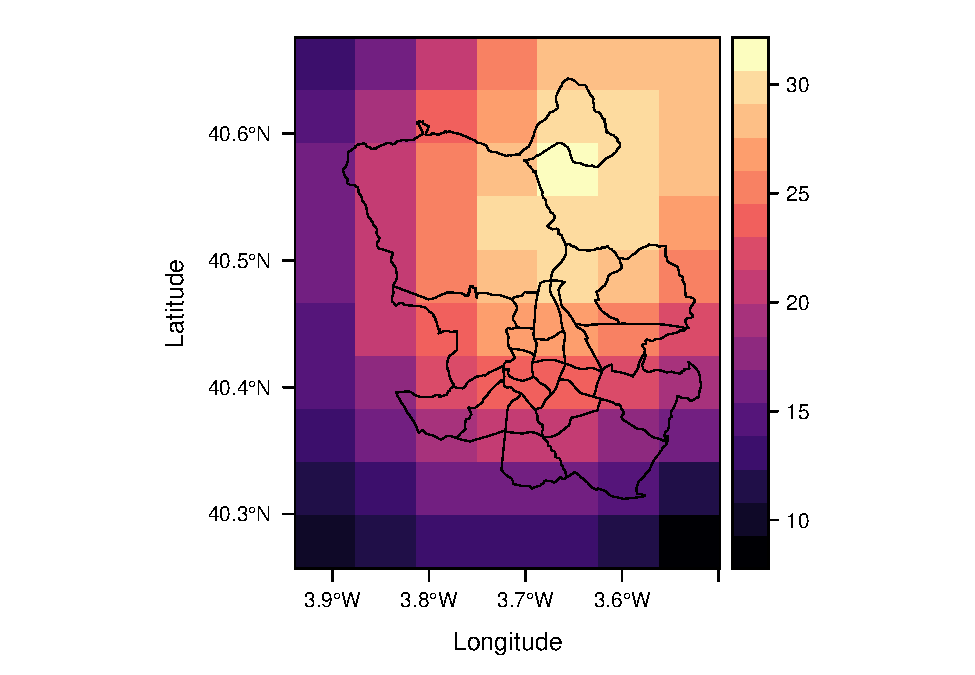
\includegraphics[scale = 0.4]{M1result.pdf}
\caption{MACC interpolated to the city grid resolution }
\label{fig:reM1}
\end{figure}

From all the models, the model 2a and model 4.3 obtained lower variance and magnitude of errors in terms of RMSE and MAE. The differences in accuracy between all the random forest models are small. 

\begin{table}[tbp]
\centering
\begin{tabular}{ c l l c c c c c}
  \toprule
 Model &Method& independent variables& Median & IQR& Mean &  RMSE& MAE \\
 \midrule
 1     &OK & \-                 & -18.29 &	22.74&	-22.20 &	28.76 &	21.13\\
 2a    &LM & MACC                  & 8.86 & 23.25     & 5.32 & 19.73 & 16.00 \\
 2b   & LM & MACC, har    &-3.21        & 26.71     & -5.87& 23.17 & 17.50  \\
 2c    &LM & MACC, har, TOD   & -3.10  & 26.68   & -5.90 & 23.09 & 17.44\\ 
 3      &UK & MACC             & -6.26 & 35.2 & -0.75 & 31.10 & 24.28\\
 4.1   &RF & DOY, MACC, TOD, har &  1.90 & 19.71 &-0.26 &19.54& 14.80 \\
 4.2a  &RF & DOY, MACC, TOD                     & 1.11&	20.97	& -2.69 &	20.13 &	15.21 \\
 4.2b  &RF & DOY(factor), MACC, TOD  & 1.17&	21.00	& -2.66 &	20.15	& 15.23 \\
 4.3   &RF & DOY, MACC              &1.09 &	21.60	& -0.60  &	20.57	& 15.76 \\
 4.4   &RF & MACC                   &0.64 &	23.60	& -1.15 &	22.21	& 16.91 \\
4.5 &RF &downscaled MACC, DOY &1.08 &21.59  &-0.61 &20.59& 15.76 \\
\bottomrule
\end{tabular}
\caption{Average of the accuracy obtained from all station measurements. MACC: halfday MACC NO2 concentration simulations. TOD: time of day (number 1 or 2 to represent day and night).
DOY: day of year (ordinal numbers from 1 to 365 to represent day of year). DOY(factor): each DOY is treated as a factor (variable). har: harmonic terms. Median: median of error, IQR: interquantile range of error, Mean: mean of error. RMSE: root mean squred error, MAE: median abolute error.
 } 
\label{table:result}
\end{table} 
 
 
\section{Discussion}

The accuracy of the model 3 is accessed by its spatial interpolation error. Because the station measurements are used in the Kriging model, the prediction at
each station are very close to the station measurements (i.e., the
prediction errors will be very small at the stations). Therefore the differences between station measurements and model prediction can not be used to assess the accuracy.  

TO BE DISCUSSED
\begin{itemize}
\item Can spatial correlation between a limited number of air quality stations be used to improve air quality prediction?

\item Does the inclusion of time series characters, such as trend and harmonic terms in a random forest model improve model prediction?
 
\item What are the strength and weakness of using  geostatistical and random forest models to predict air quality with station measurements, MACC simulation, and temporal variables? 
\end{itemize}

%\todo[inline]{I still don't quite
%  understand this. The objective of the work is to predict the
 % measures obtained in the stations, so if they are low this means
 % that we achieved the objective, isn't it? Maybe we need to discuss
  %this over skype.}

\section{Conclusion}

In summary, the linear regression model 2a and the random forest 4.3
obtain the lowest RMSE (the best accuracy and lowest
variance). Spatial correlation may be used in random forest (as
distance) to further improve the accuracy. The linear regression
models and random forest models show station measurements can be used to improve the prediction from spatially interpolate MACC simulations without using any station measurements.
Besides the model  4.4, which only uses the MACC simulations and has obtained a worse accuracy comparing to other random forest models, the differences between using different temporal variables in random forest method are small, indicating the random forest method can automatically find the cyclical patterns and the pre-assumed cyclical varioubles of time series is unecessary. 

\section *{appendix}

The R package \texttt{ranger} is used to perform random forest. In
this study, it is found that \texttt{ranger} is faster than the
\texttt{randomForest} package.  
It might be of interest to compare different randomforest
implementaions.

\bibliographystyle{plain}
\bibliography{references}
\end{document}




\todo{I moved the four subsections about the results obtained by each
  model to this section. In my opinion, they definitely need to be
  expanded with more details about the different results and with
  critical asertions on them.}



\subsection{MACC interpolation} 
Interpolation of MACC forecasts: Strong spatial correlation are shown
between MACC forecasts for all the parameters. Relatively low
interpolation error.

\subsection{Linear and nonlinear regression model}  
The linear relationship between MACC forecasts and station
measurements of NO2 is not so strong. Polynomial model of different
orders and a general additive model were attempted. Harmonic terms
were also used to fit the model.

\subsection{Universal Kriging model}  
There are 24 stations available for NO2 and we calculated pooled
residual variograms to draw more information from historical
measurements; however, the sample size is still small for identifying
spatial correlations. 
Three possible reasons are: 1) there are too few observations (stations), 2)
there is a lack of information from short-distance placed stations, 3)
due to the design of the air pollution measuring station network, the
stations are placed where the pollution is suspected to be high, e.g.,
near factories, in a canyon.   

\subsection{Random forest model}  
Random forest regression: One or more of the variables of MACC
simulation, day of year (DOY), time of day, lagged MACC simulations
and harmonic terms are used as independent variables. Random forest
methods have obtained similar results with different parameters. The
model 4.3, which uses MACC and DOY could be the most favorable random
forest model due to its simplicity and high accuracy
